\section{Bilder}
\label{sec:Bilder}

\lipsum[1]
\begin{figure}[h]
	\centering
		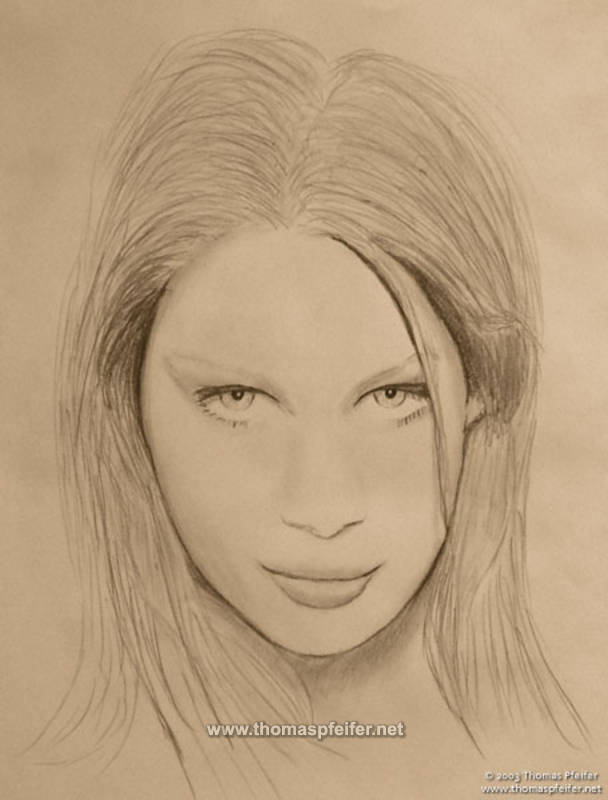
\includegraphics[width=0.50\textwidth]{bilder.jpg}
	\caption{Gesicht}
	\label{fig:bilder}
\end{figure}
\lipsum[1-2]

\subsection{Zwei Bilder nebeneinander}
\label{sec:ZweiBilderNebeneinander}

\lipsum[1]

\begin{figure}[h]
	\begin{minipage}[h]{5cm}
		\centering
			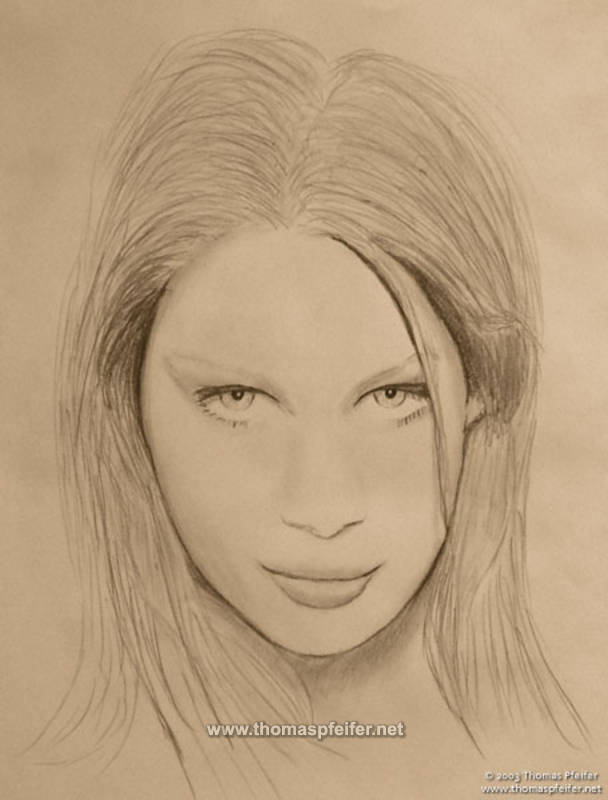
\includegraphics[width=1\textwidth]{bilder.jpg}
		\caption{Geicht 1}
		\label{gig:Gesicht1}
	\end{minipage}
	\hfill
	\begin{minipage}[h]{5cm}
		\centering
			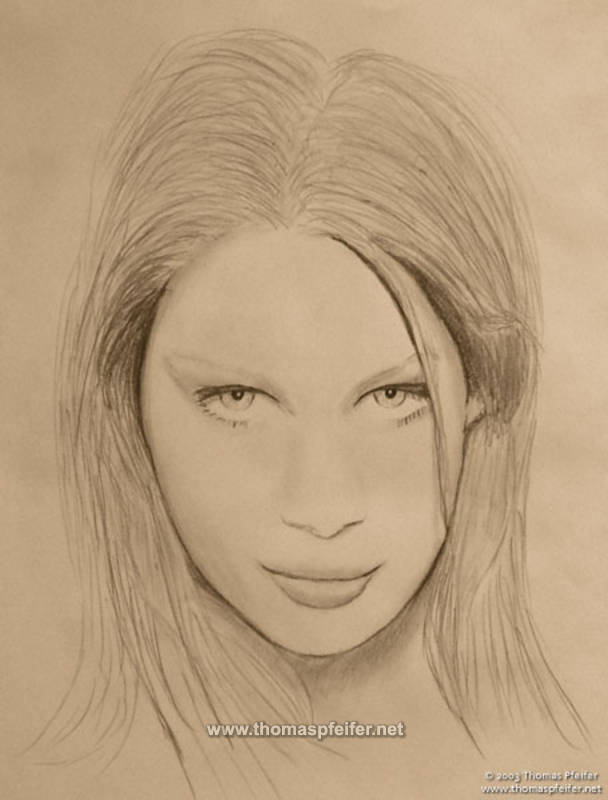
\includegraphics[width=1\textwidth]{bilder.jpg}
		\caption{Gesicht 2}
		\label{fig:Gesicht2}
	\end{minipage}
\end{figure}

\lipsum[1]

\section{Tabellen \& Listen}
\label{sec:TabellenListen}

\subsection{Tabellen}
\label{sec:Tabellen}

\begin{table*}[h]
	\centering
		\begin{tabular}{|l|c|r|}
			\hline
			\textbf{Spalte 1} & \textbf{Spalte 2} & \textbf{Spalte 3}\\
			\hline
			1 & 2 & 3 \\
			\hline
			\multirow{2}{*}{Multi}
				& Wert 2 & Wert 3 \\
				& Wert 2 & Wert 3 \\
			\hline
			z1 & z2 & z3 \\
			\hline
		\end{tabular}
	\caption{Beispieltabelle}
	\label{tab:Beispieltabelle}
\end{table*}

\subsection{Listen}
\label{sec:Listen}

\subsubsection{Ungeordnete Listen}
\label{sec:UngeordneteListen}

\begin{itemize}
	\item Element 1
	\item Element 2
	\begin{itemize}
		\item Element 3
		\begin{itemize}
			\item Element 4
		\end{itemize}
	\end{itemize}
\end{itemize}

\subsubsection{Geordnete Listen}
\label{sec:GeordneteListen}

\begin{enumerate}
	\item Element 1
	\item Element 2
	\begin{enumerate}
		\item Element 3
		\begin{enumerate}
			\item Element 4
			\item Element 5
		\end{enumerate}
		\item Element 6
	\end{enumerate}
\end{enumerate}

\subsubsection{Beschreibungen}
\label{sec:Beschreibungen}

\begin{description}
	\item[Schlagwörter] stehen am Anfang einer Zeile und werden jeweils fett gedruckt, während die zugehörige \dots
	\item[Beschreibung] dahinter in normaler Schrift erscheint.
\end{description}


